% -*- mode: latex; fill-column: 65; -*-
\documentclass[aps, pra, preprint]{revtex4-1}
\usepackage{amssymb}
\usepackage{amsmath}
\usepackage{siunitx}
\usepackage[colorinlistoftodos,prependcaption,textsize=tiny]{todonotes}
\usepackage{blindtext}
\presetkeys%
    {todonotes}%
    {inline,backgroundcolor=yellow}{}

\bibliographystyle{apsrev4-1}

\newcommand{\hzero}{H_0}
\newcommand{\phicap}{\varphi_{\rm cap}}
\newcommand{\phiwall}{\varphi_{\rm wall}}


\begin{document}

\title{Computational analysis of laser cooling of ultra-cold ions
  in Penning traps
}

\author{Dominic Meiser}
\affiliation{Trimble Inc, Boulder, 4730 Walnut Street, Suite 201,
Boulder, CO 80301, USA.}
\author{John J Bollinger}
\affiliation{National Institute of Standards and Technology,
Boulder, Colorado 80305, USA.}

\begin{abstract}
  We develop a computational model for the analysis of ultra-cold
  ions in Penning traps. We extensively verify our finite
  temperature model by comparison with zero temperature models
  and by considering well understood limiting cases. We validate
  the model by comparison with experimental results for
  single-plane to multi-plane instabilities of the ion crystal
  and by comparison with experimentally observed spectra for the
  out-of-plane modes of the ion crystal.
  We then use our model to study the temperature of the in-plane
  modes which are experimentally challenging to access. We find
  that ...\todo{Findings for in-plane modes}
  \todo{Optimization of laser cooling parameters}
\end{abstract}

\maketitle


Ultra-cold ions in Penning traps enable studies at the forefront
of atomic physics\todo{references}, quantum
science\todo{references}, and condensed matter
physics\todo{references}. Many of these studies benefit from
lower temperatures. Colder temperatures increase the crystal
stability, decrease dephasing rates, and they can increase
interrogation times. Improved crystal stability has the potential
to enable optical access to individual lattice sites which could
lead to higher fidelity state preparation and state readout for quantum
metrology\todo{references} and quantum simulation
experiments\todo{references}.

The primary means of cooling ions in Penning traps are various
forms of laser cooling including Doppler cooling and side band
cooling. While the basic principles of laser cooling for
ultra-cold ions is the same as for neutral atoms in
magneto-optical traps there are also significant differences that
can make it challenging to understand the experimentally achieved
ion temperature, cooling limits, cooling and heating mechanisms,
and that can make it more challenging to optimize the cooling
laser parameters such as intensity and detuning as well as the
cooling laser geometry.

A major difference compared to neutral atom experiments is that
ions in Penning traps move in a magnetic field several Tesla
strong. The Lorentz force in the magnetic field forces the ions
into circular orbits with a cyclotron frequency on the order of a
few hundred kilo Hertz. The rotation of the ions in the magnetic
field means that the ions velocity periodically changes direction
relative to any cooling laser beams that are stationary in the
laboratory frame of reference. A second major difference is the
strong interaction between the ions due to the Coulomb force. The
Coulomb force couples the ions into collective modes of motion.
In contrast to the cooling dynamics of neutral atoms---which is
largely a single particle phenomenon---it is necessary to take
the collective nature of the ion motion into account to fully
understand the cooling dynamics of ultra-cold ions in Penning
traps.

To help us better understand the dynamics of ultra-cold ions in
Penning traps we have developed computer simulations that allow
us to quantitatively track the dynamics of the ions over time
scales from fractions of a nano-second all the way to milli
seconds and seconds. In this paper we demonstrate the validity of
these simulations by comparison with other simulations as well as
by comparison with experimental data. We then use these
simulations to study the spectra of the out-of-plane and in-plane
modes of motion of ultra-cold ions. We compute the temperatures
of these modes and determine optimal laser cooling parameters.

{\bf Who has studied cooling dynamics before? How did they do
it?} Need a significant review of the existing literature here.
Some key workds: Dan Dubin, Dave Wineland and JJ Bollinger,
Molecular Dynamics simulations, analytical studies, fluid models,
tracking codes, particle methods, PIC, Direct Simulation Mode
Carlo (DSMC).

The rest of this article is organized as follows. We begin by
discussing the mathematical model and computational approach
underlying our analysis in section~\ref{sec:model}. We then
verify our simulations by comparison with zero temperature models
in section~\ref{sec:verification}. Specifically, we compare
steady state solutions and  spectra for the out-of-plane modes of the
ion crystal. We validate the simulations by comparison with
experimental results for the single-plane to multi-plane
instability in section~\ref{sec:validation}. In
section~\ref{sec:inplanemodes} we consider the in-plane modes and
in section~\ref{sec:optimization} we present a numerical
optimization of the laser cooling parameters and we discuss the
coldest temperatures achievable with Doppler cooling. We wrap up
with section~\ref{sec:conclusion}


\section{Model and computational algorithm}
\label{sec:model}

In this section we describe our mathematical model as well as the
computational techniques used in our numerical simulations.


\subsection{Mathematical model}

We treat the ions as classical point particles with 
velocity $\mathbf{v}_i$ and position $\mathbf{x}_i$. The motion
of the ions is governed by the Hamiltonian
\begin{equation}
  H = \hzero + \sum_{i=1}^N q_i\varphi(\mathbf{x}_i)\;,
\end{equation}
where the free Hamiltonian
\begin{equation}
  \hzero =
  \sum_{i=1}^N \frac{1}{2m_i}\left(
    \mathbf{p}_i -
    q_i\mathbf{A}(\mathbf{x}_i) \right)^2 
  \label{eqn:total_hamiltonian}
\end{equation}
includes the vector potential $\mathbf{A}$ for the axial magnetic
field in the Penning trap. We choose our coordinate system such
that the Penning trap magnetic field $\mathbf{B} =
\mathbf{\nabla}\times \mathbf{A}$ is parallel to the $z$ axis.
With that choice of coordinate system we have $\mathbf{A} =
yB_z\mathbf{\hat x}$ with $\mathbf{\hat x}=\mathbf{x}/x$ the unit
vector along $\mathbf{x}$. In Eqn.~\eqref{eqn:total_hamiltonian},
$N$ is the number of ions in the trap, $m_i$ is the mass of ion
$i$, $q_i$ its charge, and the electrostatic potential
\begin{equation}
  \varphi(\mathbf{x}_i) =
  \phicap(\mathbf{x}_i) +
  \phiwall(\mathbf{x}_i) +
  \sum_{\substack{j=1\\j\neq i}}^N
  \frac{1}{4\pi\varepsilon_0}\
  \frac{q_j}{\left| \mathbf{x_i} - \mathbf{x_j} \right|}
\end{equation}
contains the potential $\phicap$ due to the end-cap electrodes in
the Penning trap, the rotating wall potential $\phiwall$, and the
Coulomb potential for the interaction between the ions. In the
vicinity of the ion crystal the end-cap and rotating wall
potentials are well approximated by harmonic potentials. We
parametrize them as
\begin{equation}
  \phicap(\mathbf{x}) +\phiwall(\mathbf{x}) =\frac{1}{2}k_z z^2 - 
\frac{1}{2} \left(k_x x_r^2 + k_y y_r^2\right)
\end{equation}
where
\begin{equation}
k_x=\left(\frac{1}{2}+\delta\right)k_z,\qquad 
k_y=\left(\frac{1}{2}-\delta\right)k_z\;,
\end{equation}
The dimensionless parameter $\delta$ characterizes the strength
of the rotating wall potential. The coordinates of the ions in
the rotating frame $[x_r, y_r]^T$ are given by
\begin{equation}
\left[
\begin{array}{c}
x_r\\
y_r
\end{array}\right] =
\left[
\begin{array}{cc}
\cos(\vartheta(t)) & -\sin(\vartheta(t))\\
\sin(\vartheta(t)) & \cos(\vartheta(t))
\end{array}\right]
\left[\begin{array}{c}
x\\
y
\end{array}\right]\;.
\end{equation}
The phase of the rotating wall potential is
\begin{equation}
\vartheta(t)=\omega_R t+\vartheta_0\;.
\end{equation}

In addition to the conservative dynamics described by the
Hamiltonian the ions are subject to radiation pressure forces due
the cooling lasers. We describe the radiation pressure force
using a stochastic model. We discuss this model in more detail
when we consider the computational integration of the ion motion
in the next section.


\subsection{Numerical algorithm for time propagation}

To numerically integrate the motion of the ions we employ a split
step algorithm as is customary in e.g. molecular dynamics
simulations. To advance the positions and velocities of the ions
$\{\mathbf{x}_i, \mathbf{v}_i\}$
from time $t$ to $t + \Delta t$ we use the update formula
\begin{equation}
  \{\mathbf{x}_i, \mathbf{v}_i\}(t+\Delta t) =
  U_{0}(\Delta t /2)
  U_{\rm kick}(t + \Delta t / 2; \Delta t)
  U_{0}(\Delta t /2)
  \{\mathbf{x}_i, \mathbf{v}_i\}(t)\;.
\end{equation}
In this formula, $U_{0}(\Delta t/2)$ is the time evolution
operator corresponding to $\hzero$ that advances the state of
the ions for a time interval of duration $\Delta t / 2$. Since
the free Hamiltonian contains just the kinetic energy of the ions
and the Lorentz force due to the axial magnetic field the motion
generated by $U_{0}$ is the well known circular Larmor
procession,
\begin{eqnarray}
  \mathbf{x}_i(t + \Delta t / 2) &=&
                                   \mathbf{x}_i(t)+\\
  &&
      \left[\begin{array}{ccc}
        s & c - 1 & 0\\
        -c + 1 & s & 0\\
        0 & 0 & \omega_B\Delta t / 2
      \end{array}\right]\frac{\mathbf{v}_i(t)}{\omega_B}\;,\nonumber\\
  \mathbf{v}_i(t+\Delta t/2) &=&\mathbf{v}_i(t) + \left[\begin{array}{ccc}
        c & -s & 0\\
        s & c & 0\\
        0 & 0 & 0
      \end{array}\right]\mathbf{v}_i(t)\;,
\end{eqnarray}
where
\begin{equation}
  s = \sin(\omega_B \Delta t / 2)
\end{equation}
and
\begin{equation}
  c = \cos(\omega_B \Delta t / 2)
\end{equation}
with $\omega_B=B_zq/m$ the Lamor precession frequency.

The time evolution operator $U_{\rm kick}(t + \Delta t/2; \Delta
t)$ corresponds to the interaction with the forces due to the
electrostatic potential as well as the radiation pressure forces
due to laser cooling. This operator is time dependent due to the
rotating wall potential and the radiation pressure forces. We
evaluate it at the mid-point of the time interval, $t + \Delta t
/ 2$. The operator $U_{\rm kick}$ changes the momenta of the
particles only,
\begin{eqnarray}
  \{\mathbf{x}_i, \mathbf{p}_i\}(t + \Delta t)
  &=& U_{\rm kick}(t + \Delta t /2; \Delta t)
    \{\mathbf{x}_i, \mathbf{p}_i\}(t)\\
  &=&\left\{
      \mathbf{x}_i(t),
      \mathbf{p}_i(t) +
      \Delta t q_i \mathbf{E}(t + \Delta t / 2, \mathbf{x}_i) +
      \Delta \mathbf{p}_i^{\rm laser}
      \right\}\;.
\end{eqnarray}
The kick due to the electric field is given by $\Delta t
q_i\mathbf{E}(t+\Delta t /2,\mathbf{x}_i) = -\Delta t
q_i\mathbf{\nabla}\varphi(\mathbf{x}_i)$.

Our model of laser cooling is based on resonance fluorescence for
a driven two-level atom. The photon scattering rate for a driven
two-level atom is given by
\begin{equation}
\dot n (\mathbf{r}, \mathbf{v}) = 
S(\mathbf{r})\frac{\gamma_0}{2\pi}
\frac{(\gamma_0/2)^2}{(\gamma_0/2)^2(1+2S(\mathbf{r}))+\Delta^2(\mathbf{v})}\;,
\end{equation}
where $\gamma_0$ is the natural linewidth of the cycling transition (in
radians per second), $S(\mathbf{r})$ is the saturation parameter, and
$\Delta(\mathbf{v})=\Delta_0 + \mathbf{k}\cdot\mathbf{v}$ is the
detuning of the cooling transition from the laser frequency including
the first order Doppler shift.  We assume that the atoms scatter photons
with this rate with Poissonian number statistics\footnote{Strictly
speaking, this is only valid in the limit of low saturation (for
$S\sim 1$ we have to take into account anti-bunching).}.  We take into
account the beam profile by multiplying the saturation parameter with a
Gaussian factor that accounts for the spatial structure of the laser,
\begin{equation}
S(\mathbf{r})=e^{-\rho^2/\sigma^2}S_0\;,
\end{equation}
where $\rho$ is the distance of the atom from the center of the beam and
$\sigma$ is the $1/e$ radius of the intensity of the beam.

To numerically simulate laser cooling we proceed as follows.
First we compute the mean number of photons scattered by ion $i$
in time interval $\Delta t$,
\begin{equation}
n_i=\dot{n}_i \Delta t\;.
\end{equation}
The velocities and positions needed for computing $\dot{n}_j$ are taken
at the center of the time step in accordance with the integration scheme
discussed above.  We then compute the actual number of photons scattered
by each ion as a Poissonian random number with mean $n_i$.  Each
ion receives a total momentum kick of 
\begin{equation}
\mathbf{\Delta p}_i = \mathbf{\Delta p_{i,{\rm absorb}}} + 
\mathbf{\Delta p_{i,{\rm emit}}}\;,
\end{equation}
where $\mathbf{\Delta p_{i,{\rm absorb}}}=n_i \hbar \mathbf{k}$ and
$\mathbf{\Delta p_{i,{\rm emit}}}$ is the recoil corresponging to $n_i$
photons scattered in random directions. To compute $\mathbf{\Delta
p_{i,{\rm emit}}}$ we generate $n_i$ vectors of length $\hbar k$
pointing in random directions.  The recoil momentum $\mathbf{\Delta
p}_{i,{\rm emit}}$ is then obtained by adding up these vectors.

This approach captures the microscopic physics of laser cooling
except for two phenomena. First, in the case of strong
saturation, $S\gtrsim 1$, quantum statistical phenomena start to
play a role. These manifest themselves in the form of
anti-bunching of the photons scattered in resonance fluorescence.
In essence, there is an anti-correlation between photon emission
events due to the fact that immediately after a photon emission
an atom is in the ground state with certainty and therefore
cannot emitt another photon right away. The other approximation
model is that we assume that the photon emission is nearly
instantaneous relative to the dynamics of the ions, i.e. the
motion is uniform during an excited state lifetime, i.e. we
assume that 
\begin{equation}
\eta\equiv\gamma_0/\omega_B\ll 1\;.
\end{equation}
In our case this ratio is approximately $\eta \sim 0.3$.



\section{Verification and validation of the dynamical
simulations}
\label{sec:VerificationAndValidation}

In this section we verify the correctness of our numerical
integration procedure. We check that the simulations converge
with the expected quadratic rate as the time step size is
reduced. We compare the temperature of laser cooled ions with the
well known text book result for Doppler cooling. We check that
the steady state obtained with a separate static zero temperature
code is a steady state of our simulations. Finally we compare
simulation results for a single-plane to multi-plane instability
with theoretical and experimental results.


\subsection{Convergence}

One of the most basic tests of the correctness of our time
integration scheme is to verify that it converges to a solution
as the time step size is reduced. To evaluate the convergence we
initialize our simulation with a steady state configuration of
127 ions shown in Fig.~\ref{fig:initial_state_top_view}. Here and
in the results discussed below we use parameters typical for the
Penning trap at NIST Boulder with a homogeneous magnetic field of
$B_z=\SI{4.4588}{\tesla}$, a trap rotation frequency of
$\omega_{\rm trap}=2\pi\times \SI{180}{\kilo \hertz}$, end cap
voltages yielding a confining potential of
$k_z=\SI{9.21}{\mega\volt/\meter^2}$, and a rotating wall
potential of $V_{\rm Wall} = \SI{1}{\volt}$ yielding
$\delta=\SI{3.5e-4}{}$.
\begin{figure}
  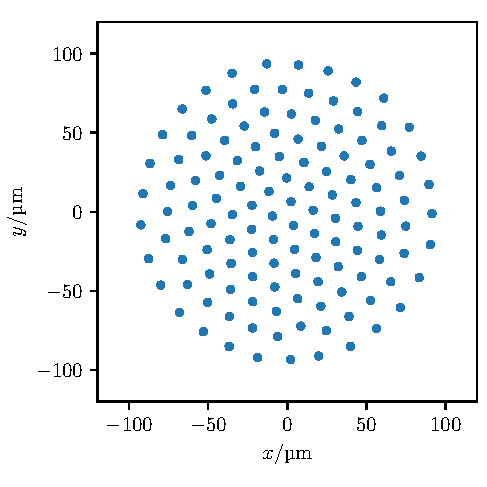
\includegraphics{./figures/fig_initial_state_top_view.pdf}
  \caption{Top view of steady state configuration of ions in
    Penning trap used for convergence study.}
  \label{fig:initial_state_top_view}
\end{figure}

Starting from this initial steady state configuration we
integrate the equations of motion for $\SI{10}{\us}$ using
different time step sizes. For each time step size we compare the
final solution with a reference solution computed using a time
step size of $\Delta t = \SI{2e-10}{\second}$. We compute the
error $\Delta x(\Delta t)$ in the simulation result
$\mathbf{x}(\Delta t)$ as the average Euclidian distance between
the reference solution $\mathbf{x}^{\rm
  ref}=\mathbf{x}(\SI{2.0e-10}{\second})$,
\begin{equation}
  \Delta x(\Delta t) =
  \sqrt{N^{-1}\sum_{i=1}^N\left(
      \mathbf{x}_i(\Delta t)-\mathbf{x}_i^{\rm ref}\right)^2}\;.
\end{equation}

The result is shown in Fig.~\ref{fig:convergence}. The error
decreases quadratically for time step sizes below approximately
$\SI{1.0e-7}{\second}$. At time step size of $\Delta t =
\SI{1}{\nano\second}$ the mean position error of the ions is
$\Delta x(\SI{1}{\nano\second})\approx \SI{1}{\nano\meter}$. For
reference, during this time interval the ions move on the order
of $\SI{1}{\milli\meter}$, i.e. the ion motion is integrated with
a relative error on the order of $\SI{1.0e-6}{}$. For time step
sizes greater than $\Delta t\approx 1.0e-7$ the integrator can be in
resonance with some of the vibrational eigen modes of the system.
Whenever the integrator is in resonance errors can grow
indefinitely. While damping forces such as laser cooling can
broaden the resonances and limit the growth of errors it is best
to stick to time step sizes that are smaller than $\Delta t =
\SI{1.0e-7}{\second}$. Results quoted in this paper were obtained
with $\Delta t = \SI{1}{\nano\second}$ unless noted otherwise.
\begin{figure}
  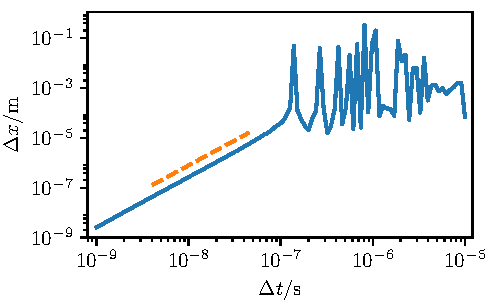
\includegraphics{./figures/fig_convergence.pdf}
  \caption{Integration errors as a function of time step size for
    a total time integration time of $T=\SI{10}{\us}$ for a
    typical Penning trap simulation. The dashed orange line is a
    quadratic for orientation. See text for details.}
  \label{fig:convergence}
\end{figure}


\subsection{Free space laser cooling}

As a simple test of our laser cooling model we simulate free
space laser cooling. Free space means that the ions are not
subject to any trapping or magnetic fields.
Figure~\ref{fig:FreeSpaceCooling} shows the velocities of five
Beryllium ions subject to laser cooling. The atoms start with a
velocity of $v_x=\SI{10}{\meter/\second}$. The ions are
irradiated by three counter propagating pairs of laser beams
along the Cartesian axis $\pm\hat{\mathbf{x}}$,
$\pm\hat{\mathbf{y}}$, and $\pm\hat{\mathbf{z}}$. The lasers have
uniform intensities of $S=0.1$ and are detuned by $0.5\gamma_0$
to the red of the cycling transition at $313{\rm nm}$. The atomic
linewidth is $\gamma_0=2\pi\times \SI{19}{\mega\hertz}$.

\begin{figure}
  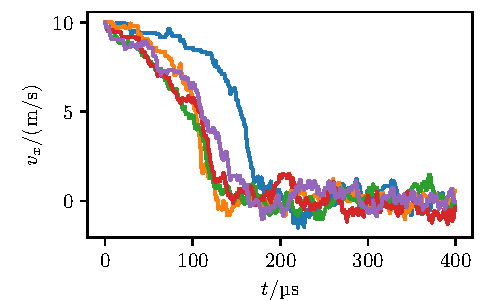
\includegraphics{./figures/fig_laser_cooling.pdf}
  \caption{Trajectories of Beryllium ions undergoing laser
    cooling.}
  \label{fig:FreeSpaceCooling}
\end{figure}
As can be seen in Fig.~\ref{fig:FreeSpaceCooling}, the ions are
cooled to the Doppler limit. The root mean squared velocity at the Doppler
temperature is
\begin{equation}
\sqrt{\langle v_x^2\rangle} = \frac{\hbar \gamma_0}{m} \approx
\SI{0.87}{\meter/\second}\;,
\end{equation}
which is in good agreement with the value of $\sqrt{\langle
  v_x^2\rangle}=\SI{1.16}{\meter/\second}$ found in our
simulation.


\subsection{Single-plane to multi-plane instability}
\label{sec:validation}

When the rotation frequency of the ion crystal in the Penning
trap is increased the radial confining potential generated by the
axial magnetic field becomes stronger and stronger. Eventually
the single plane crystal configuration shown in
Fig.~\ref{fig:initial_state_top_view} becomes unstable and it
becomes energetically favourable for the ions to arrange
themselves in multiple crystal planes. The frequency at which
this instability occurs is well understood
theoretically\todo{references} and has been carefully
characterized experimentally\todo{references}. We simulate the
transition here to gain further confidence in the correctness and
accuracy of our simulations. The study of the single plane
instability is also a nice illustration of the generality of our
approach.

To simulate the single-plane instability we start with the single
plane equilibrium configuration shown in
Fig.~\ref{fig:initial_state_top_view}. We then sweep the rotation
frequency of the rotating wall potential from
$\omega(t=0)=2\pi\times\SI{185}{\kilo\hertz}$ to
$\omega(t=\SI{1}{\milli\second})=2\pi\times\SI{205}{\kilo\hertz}$ with
a sweep rate of $d\omega/dt =
\SI{20}{\kilo\hertz/\milli\second}$. After holding the rotation
frequency there for $\SI{1}{\milli\second}$ we sweep back to the
original frequency with
$d\omega/dt=-\SI{20}{\kilo\hertz/\milli\second}$. The frequency
sweep $\omega(t)$ is shown in the inset in
Fig.~\ref{fig:single_plane_instability}.

During this sweep sequence we apply an artificial damping to the
ion motion in order to keep the ions close to a minimal energy
configuration. The damping is given by
\begin{eqnarray}
  \frac{v_z}{dt}&=&-\kappa_z v_z\;,\\
  \frac{v_\vartheta}{dt}&=&-\kappa_\vartheta\left( v_\vartheta -
                            \omega\left| \mathbf{r} \right| \right)\;.
\end{eqnarray}
For the simulations discussed here we use
$\kappa_z=\SI{1e6}{\second^{-1}}$ and
$\kappa_\vartheta=\SI{5e6}{\second^{-1}}$. We use these
artificial damping terms instead of a more physically accurate
laser cooling model so as to not complicate the discussion
unnecessarily.

Figure~\ref{fig:single_plane_instability} shows the thickness
\begin{equation}
  \Delta z=\sqrt{N^{-1}\sum_{i=1}^N z_i^2}
\end{equation}
of the ion crystal. As the rotation frequency increases the
single plane configuration becomes unstable at $\omega\approx
194\times 2\pi\si{\kilo\hertz}$. The thickness of the crystal
continuous to increase as more and more ions are ``squeezed'' out
of the $z=0$ plane.

\begin{figure}
  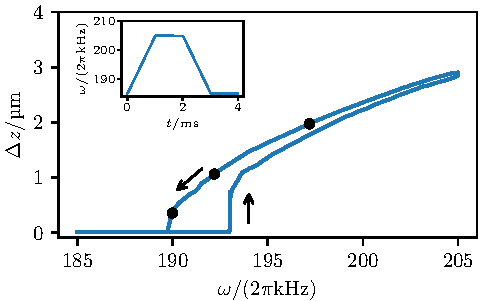
\includegraphics{./figures/fig_single_plane_instability.pdf}
  \caption{Thickness of ion crystal as a function of the rotation
    frequency. The arrows indicate the sweep direction of the
    rotation frequency for the two thickness traces. The black
    dots indicate the rotation frequencies at which the side
    views in Fig.~\ref{fig:side_views_single_plane_instability}
    are computed. The inset shows the rotation frequency as a
    function of time during the sweep.}
  \label{fig:single_plane_instability}
\end{figure}
As the rotation frequency decreases the ions move back to the
$z=0$ plane and the thickness of the crystal decreases. The
thickness of the crystal lags behind the true equilibrium
thickness due to the finite sweep rate. There is no bistability
in this system. Eventually at $\omega\approx 190\times
2\pi\si{\kilo\hertz}$ the crystal is a single plane of ions again.

Figure~\ref{fig:side_views_single_plane_instability} shows a side
view of the ion crystal during the down sweep of the rotation
frequency. These figures illustrate the arrangement of the ions
in three planes. It shows how more and more ions ``fit'' into the
$z=0$ crystal plane. Just above the transition frequency only a
small zone around $x=y=0$ is unstable.
\begin{figure}
  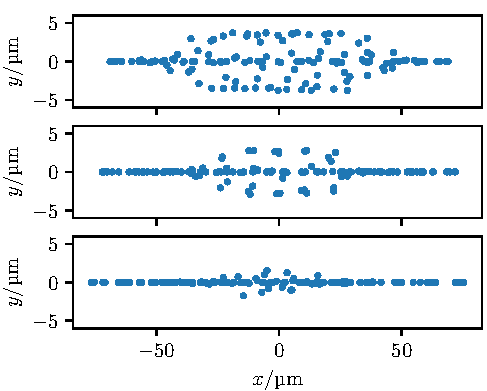
\includegraphics{./figures/fig_side_views_single_plane_instability.pdf}
  \caption{Side views of ion crystal as the rotation frequency is
    reduced to the single plane instability frequency. The
    rotation frequencies at which these side views are computed
    are indicated by the black dots in
    Fig.~\ref{fig:single_plane_instability}.}
  \label{fig:side_views_single_plane_instability}
\end{figure}


\section{Finite temperature mode analysis}

\subsection{Out-of-plane modes}

\subsection{In-plane modes}


\section{In-plane modes}
\label{sec:inplanemodes}


\section{Optimization of laser cooling parameters}
\label{sec:optimization}


\section{Conclusion}
\label{sec:conclusion}

\bibliography{cooling_bibliography}

\end{document}
